\documentclass{standalone}
\usepackage{tikz}
\usetikzlibrary{patterns, positioning}
\usepackage[sfdefault]{ClearSans} %% option 'sfdefault' activates Clear Sans as the default text font
\usepackage[T1]{fontenc}

\begin{document}
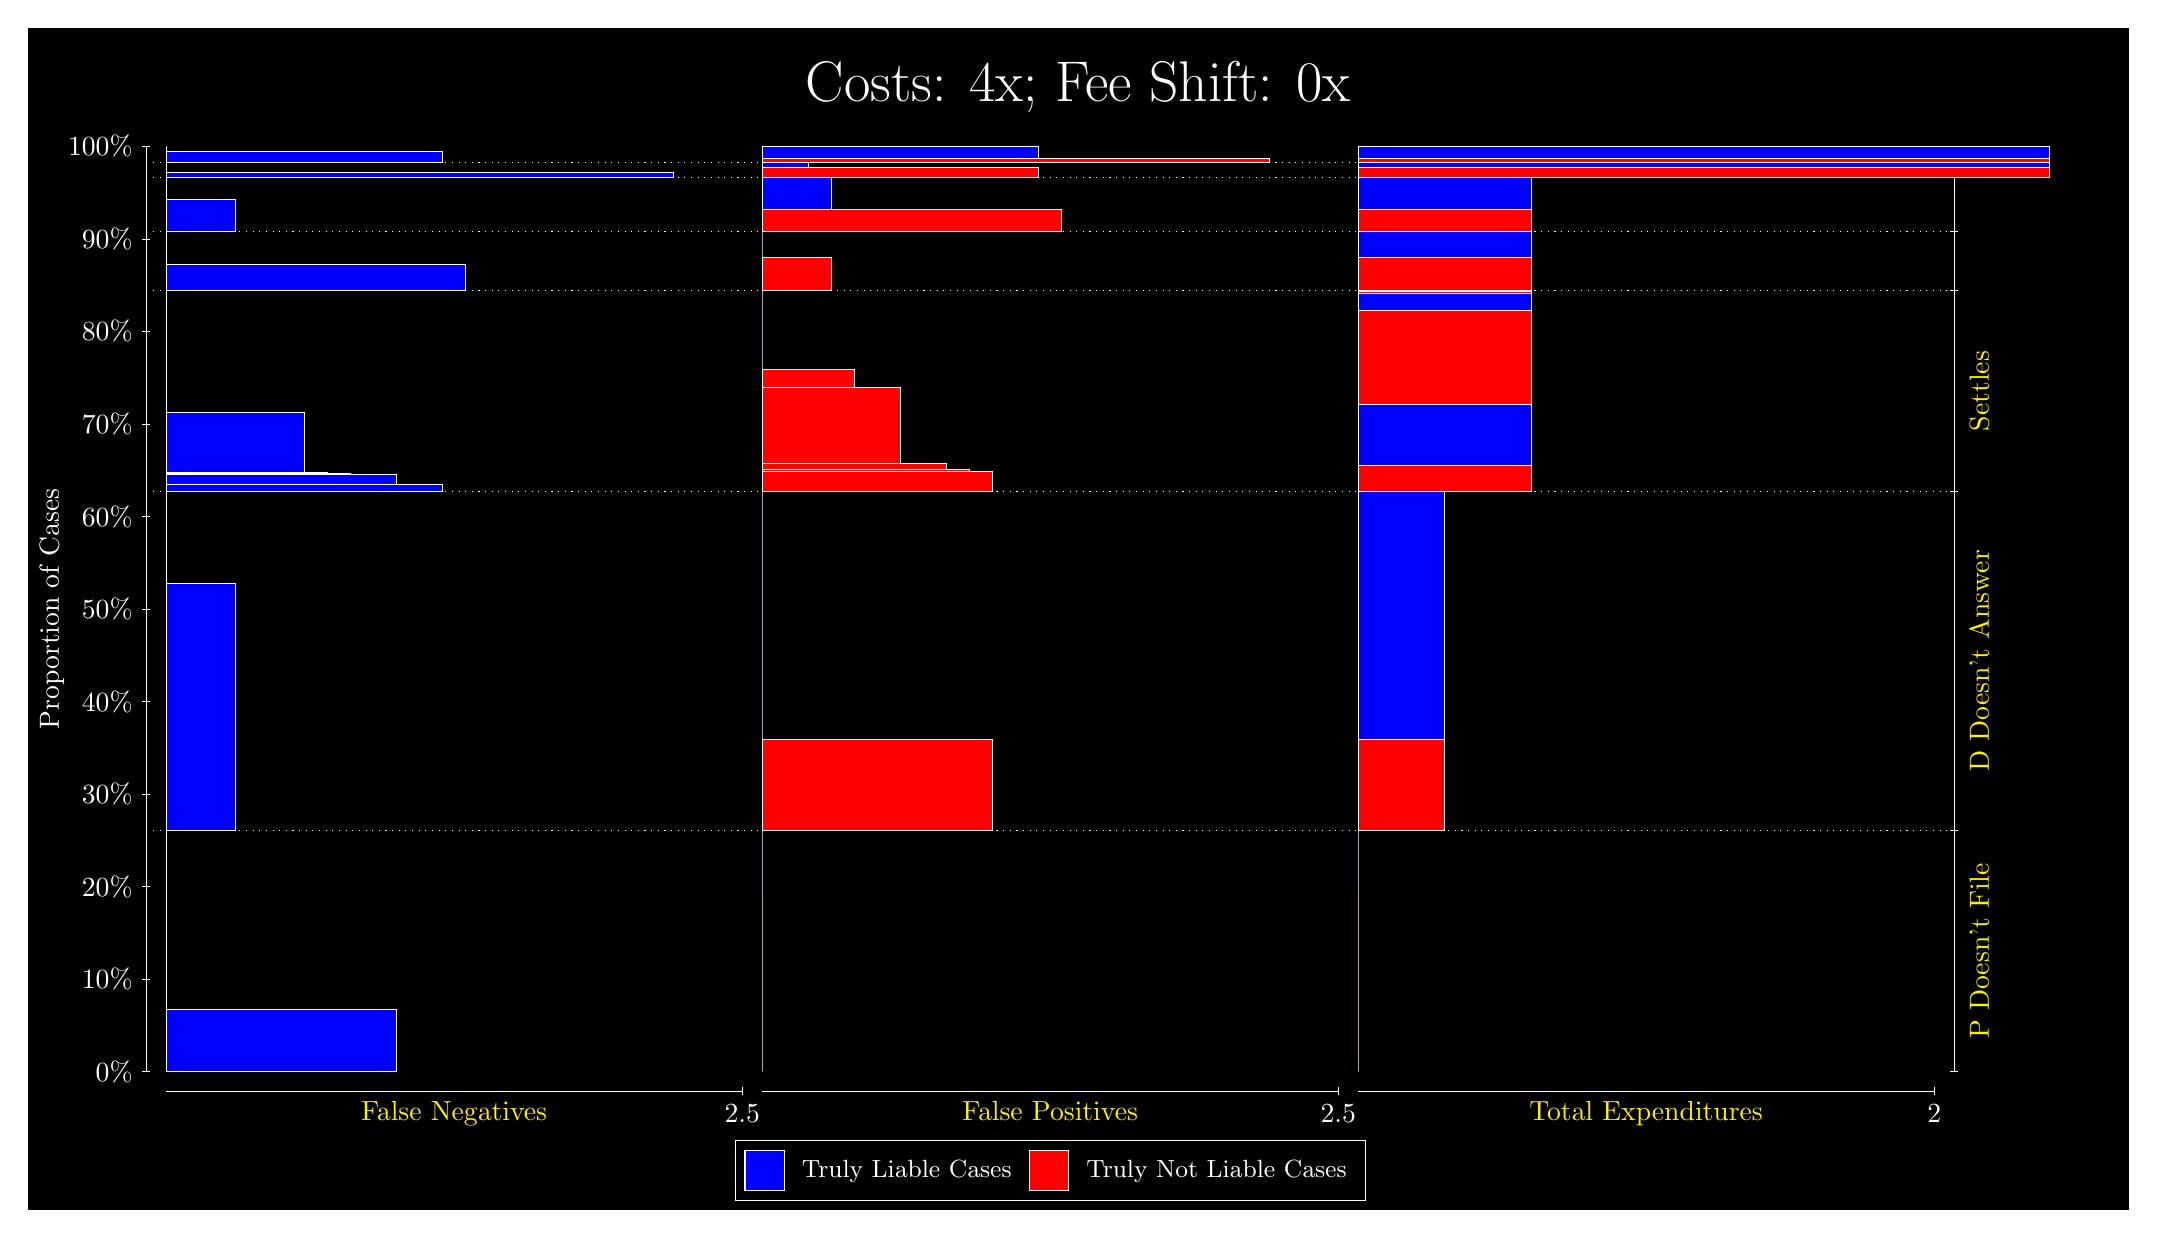
\begin{tikzpicture}
\draw[fill=black] (0,0) rectangle (26.667,15);
\draw[text=white] (0,13.5) rectangle (26.667,15) node[midway] {\huge Costs: 4x; Fee Shift: 0x};
\draw[white, very thin] (1.5,1.75) -- (1.5,13.5);
\node[rotate=90, text=white, anchor=center] at (0.3, 7.625) {Proportion of Cases};
\draw[white, very thin] (1.45,1.75) -- (1.55,1.75);
\node[text=white, anchor=east] at (1.45, 1.75) {0\%};
\draw[white, very thin] (1.45,2.925) -- (1.55,2.925);
\node[text=white, anchor=east] at (1.45, 2.925) {10\%};
\draw[white, very thin] (1.45,4.1) -- (1.55,4.1);
\node[text=white, anchor=east] at (1.45, 4.1) {20\%};
\draw[white, very thin] (1.45,5.275) -- (1.55,5.275);
\node[text=white, anchor=east] at (1.45, 5.275) {30\%};
\draw[white, very thin] (1.45,6.45) -- (1.55,6.45);
\node[text=white, anchor=east] at (1.45, 6.45) {40\%};
\draw[white, very thin] (1.45,7.625) -- (1.55,7.625);
\node[text=white, anchor=east] at (1.45, 7.625) {50\%};
\draw[white, very thin] (1.45,8.8) -- (1.55,8.8);
\node[text=white, anchor=east] at (1.45, 8.8) {60\%};
\draw[white, very thin] (1.45,9.975) -- (1.55,9.975);
\node[text=white, anchor=east] at (1.45, 9.975) {70\%};
\draw[white, very thin] (1.45,11.15) -- (1.55,11.15);
\node[text=white, anchor=east] at (1.45, 11.15) {80\%};
\draw[white, very thin] (1.45,12.325) -- (1.55,12.325);
\node[text=white, anchor=east] at (1.45, 12.325) {90\%};
\draw[white, very thin] (1.45,13.5) -- (1.55,13.5);
\node[text=white, anchor=east] at (1.45, 13.5) {100\%};

\draw[white, very thin] (24.457,1.75) -- (24.457,13.5);
\draw[white, very thin] (24.407,1.75) -- (24.507,1.75);
\node[anchor=west] at (24.407, 1.75) {};
\draw[white, very thin] (24.407,4.8132) -- (24.507,4.8132);
\node[anchor=west] at (24.407, 4.8132) {};
\draw[white, very thin] (24.407,9.1156) -- (24.507,9.1156);
\node[anchor=west] at (24.407, 9.1156) {};
\draw[white, very thin] (24.407,11.671) -- (24.507,11.671);
\node[anchor=west] at (24.407, 11.671) {};
\draw[white, very thin] (24.407,12.418) -- (24.507,12.418);
\node[anchor=west] at (24.407, 12.418) {};
\draw[white, very thin] (24.407,13.108) -- (24.507,13.108);
\node[anchor=west] at (24.407, 13.108) {};
\draw[white, very thin] (24.407,13.293) -- (24.507,13.293);
\node[anchor=west] at (24.407, 13.293) {};
\draw[white, very thin] (24.407,13.5) -- (24.507,13.5);
\node[anchor=west] at (24.407, 13.5) {};

\draw[white, very thin, fill=blue] (1.75,1.75) rectangle (4.6775,2.535);
\draw[white, very thin, fill=red] (1.75,2.535) rectangle (1.75,4.8132);
\draw[white, very thin, fill=blue] (1.75,4.8132) rectangle (2.6283,7.9569);
\draw[white, very thin, fill=red] (1.75,7.9569) rectangle (1.75,9.1156);
\draw[white, very thin, fill=blue] (1.75,9.1156) rectangle (5.2631,9.2102);
\draw[white, very thin, fill=blue] (1.75,9.2102) rectangle (4.6775,9.3294);
\draw[white, very thin, fill=blue] (1.75,9.3294) rectangle (4.092,9.3468);
\draw[white, very thin, fill=blue] (1.75,9.3468) rectangle (3.7993,9.3614);
\draw[white, very thin, fill=blue] (1.75,9.3614) rectangle (3.5065,10.121);
\draw[white, very thin, fill=red] (1.75,10.121) rectangle (1.75,11.671);
\draw[white, very thin, fill=blue] (1.75,11.671) rectangle (5.5558,11.996);
\draw[white, very thin, fill=red] (1.75,11.996) rectangle (1.75,12.418);
\draw[white, very thin, fill=blue] (1.75,12.418) rectangle (2.6283,12.826);
\draw[white, very thin, fill=red] (1.75,12.826) rectangle (1.75,13.108);
\draw[white, very thin, fill=blue] (1.75,13.108) rectangle (8.1906,13.165);
\draw[white, very thin, fill=red] (1.75,13.165) rectangle (1.75,13.293);
\draw[white, very thin, fill=blue] (1.75,13.293) rectangle (5.2631,13.443);
\draw[white, very thin, fill=red] (1.75,13.443) rectangle (1.75,13.5);
\draw[white, very thin, fill=red] (9.3189,1.75) rectangle (9.3189,4.0282);
\draw[white, very thin, fill=blue] (9.3189,4.0282) rectangle (9.3189,4.8132);
\draw[white, very thin, fill=red] (9.3189,4.8132) rectangle (12.246,5.9719);
\draw[white, very thin, fill=blue] (9.3189,5.9719) rectangle (9.3189,9.1156);
\draw[white, very thin, fill=red] (9.3189,9.1156) rectangle (12.246,9.3784);
\draw[white, very thin, fill=red] (9.3189,9.3784) rectangle (11.954,9.4047);
\draw[white, very thin, fill=red] (9.3189,9.4047) rectangle (11.661,9.4772);
\draw[white, very thin, fill=red] (9.3189,9.4772) rectangle (11.075,10.438);
\draw[white, very thin, fill=red] (9.3189,10.438) rectangle (10.49,10.665);
\draw[white, very thin, fill=blue] (9.3189,10.665) rectangle (9.3189,11.671);
\draw[white, very thin, fill=red] (9.3189,11.671) rectangle (10.197,12.092);
\draw[white, very thin, fill=blue] (9.3189,12.092) rectangle (9.3189,12.418);
\draw[white, very thin, fill=red] (9.3189,12.418) rectangle (13.125,12.699);
\draw[white, very thin, fill=blue] (9.3189,12.699) rectangle (10.197,13.108);
\draw[white, very thin, fill=red] (9.3189,13.108) rectangle (12.832,13.236);
\draw[white, very thin, fill=blue] (9.3189,13.236) rectangle (9.9044,13.293);
\draw[white, very thin, fill=red] (9.3189,13.293) rectangle (15.759,13.351);
\draw[white, very thin, fill=blue] (9.3189,13.351) rectangle (12.832,13.5);
\draw[white, very thin, fill=red] (16.888,1.75) rectangle (16.888,4.0282);
\draw[white, very thin, fill=blue] (16.888,4.0282) rectangle (16.888,4.8132);
\draw[white, very thin, fill=red] (16.888,4.8132) rectangle (17.986,5.9719);
\draw[white, very thin, fill=blue] (16.888,5.9719) rectangle (17.986,9.1156);
\draw[white, very thin, fill=red] (16.888,9.1156) rectangle (19.083,9.4509);
\draw[white, very thin, fill=blue] (16.888,9.4509) rectangle (19.083,10.228);
\draw[white, very thin, fill=red] (16.888,10.228) rectangle (19.083,11.416);
\draw[white, very thin, fill=blue] (16.888,11.416) rectangle (19.083,11.63);
\draw[white, very thin, fill=red] (16.888,11.63) rectangle (19.083,11.656);
\draw[white, very thin, fill=blue] (16.888,11.656) rectangle (19.083,11.671);
\draw[white, very thin, fill=red] (16.888,11.671) rectangle (19.083,12.092);
\draw[white, very thin, fill=blue] (16.888,12.092) rectangle (19.083,12.418);
\draw[white, very thin, fill=red] (16.888,12.418) rectangle (19.083,12.699);
\draw[white, very thin, fill=blue] (16.888,12.699) rectangle (19.083,13.108);
\draw[white, very thin, fill=red] (16.888,13.108) rectangle (25.67,13.236);
\draw[white, very thin, fill=blue] (16.888,13.236) rectangle (25.67,13.293);
\draw[white, very thin, fill=red] (16.888,13.293) rectangle (25.67,13.351);
\draw[white, very thin, fill=blue] (16.888,13.351) rectangle (25.67,13.5);
\draw[white, dotted] (1.5,4.8132) -- (24.457,4.8132);
\draw[white, dotted] (1.5,9.1156) -- (24.457,9.1156);
\draw[white, dotted] (1.5,11.671) -- (24.457,11.671);
\draw[white, dotted] (1.5,12.418) -- (24.457,12.418);
\draw[white, dotted] (1.5,13.108) -- (24.457,13.108);
\draw[white, dotted] (1.5,13.293) -- (24.457,13.293);
\draw[white, very thin] (1.75,1.5) -- (9.0689,1.5);
\node[text=yellow, anchor=north] at (5.4094, 1.5) {False Negatives};
\draw[white, very thin] (9.0689,1.45) -- (9.0689,1.55);
\node[text=white, anchor=north] at (9.0689, 1.45) {2.5};

\draw[white, very thin] (9.3189,1.5) -- (16.638,1.5);
\node[text=yellow, anchor=north] at (12.978, 1.5) {False Positives};
\draw[white, very thin] (16.638,1.45) -- (16.638,1.55);
\node[text=white, anchor=north] at (16.638, 1.45) {2.5};

\draw[white, very thin] (16.888,1.5) -- (24.207,1.5);
\node[text=yellow, anchor=north] at (20.547, 1.5) {Total Expenditures};
\draw[white, very thin] (24.207,1.45) -- (24.207,1.55);
\node[text=white, anchor=north] at (24.207, 1.45) {2};

\node[text=yellow, centered, rotate=90] at (24.777, 3.2816) {P Doesn't File};
\node[text=yellow, centered, rotate=90] at (24.777, 6.9644) {D Doesn't Answer};
\node[text=yellow, centered, rotate=90] at (24.777, 10.393) {Settles};





\draw (12.978300999999998,1.5) node[draw=none] (baseCoordinate) {};
\begin{scope}[align=center]
        \matrix[scale=0.5, draw=white, below=0.5cm of baseCoordinate, nodes={draw}, column sep=0.1cm]{
            \node[rectangle, draw, minimum width=0.5cm, minimum height=0.5cm, fill=blue] {}; &
            \node[draw=none, font=\small, text=white] (B) {Truly Liable Cases}; &
            \node[rectangle, draw, minimum width=0.5cm, minimum height=0.5cm, fill=red] {}; &
            \node[draw=none, font=\small, text=white] (B) {Truly Not Liable Cases}; \\
            };
\end{scope}

\end{tikzpicture}
\end{document}